% Options for packages loaded elsewhere
\PassOptionsToPackage{unicode}{hyperref}
\PassOptionsToPackage{hyphens}{url}
%
\documentclass[
]{article}
\usepackage{amsmath,amssymb}
\usepackage{lmodern}
\usepackage{iftex}
\ifPDFTeX
  \usepackage[T1]{fontenc}
  \usepackage[utf8]{inputenc}
  \usepackage{textcomp} % provide euro and other symbols
\else % if luatex or xetex
  \usepackage{unicode-math}
  \defaultfontfeatures{Scale=MatchLowercase}
  \defaultfontfeatures[\rmfamily]{Ligatures=TeX,Scale=1}
\fi
% Use upquote if available, for straight quotes in verbatim environments
\IfFileExists{upquote.sty}{\usepackage{upquote}}{}
\IfFileExists{microtype.sty}{% use microtype if available
  \usepackage[]{microtype}
  \UseMicrotypeSet[protrusion]{basicmath} % disable protrusion for tt fonts
}{}
\makeatletter
\@ifundefined{KOMAClassName}{% if non-KOMA class
  \IfFileExists{parskip.sty}{%
    \usepackage{parskip}
  }{% else
    \setlength{\parindent}{0pt}
    \setlength{\parskip}{6pt plus 2pt minus 1pt}}
}{% if KOMA class
  \KOMAoptions{parskip=half}}
\makeatother
\usepackage{xcolor}
\usepackage[margin=1in]{geometry}
\usepackage{color}
\usepackage{fancyvrb}
\newcommand{\VerbBar}{|}
\newcommand{\VERB}{\Verb[commandchars=\\\{\}]}
\DefineVerbatimEnvironment{Highlighting}{Verbatim}{commandchars=\\\{\}}
% Add ',fontsize=\small' for more characters per line
\usepackage{framed}
\definecolor{shadecolor}{RGB}{248,248,248}
\newenvironment{Shaded}{\begin{snugshade}}{\end{snugshade}}
\newcommand{\AlertTok}[1]{\textcolor[rgb]{0.94,0.16,0.16}{#1}}
\newcommand{\AnnotationTok}[1]{\textcolor[rgb]{0.56,0.35,0.01}{\textbf{\textit{#1}}}}
\newcommand{\AttributeTok}[1]{\textcolor[rgb]{0.77,0.63,0.00}{#1}}
\newcommand{\BaseNTok}[1]{\textcolor[rgb]{0.00,0.00,0.81}{#1}}
\newcommand{\BuiltInTok}[1]{#1}
\newcommand{\CharTok}[1]{\textcolor[rgb]{0.31,0.60,0.02}{#1}}
\newcommand{\CommentTok}[1]{\textcolor[rgb]{0.56,0.35,0.01}{\textit{#1}}}
\newcommand{\CommentVarTok}[1]{\textcolor[rgb]{0.56,0.35,0.01}{\textbf{\textit{#1}}}}
\newcommand{\ConstantTok}[1]{\textcolor[rgb]{0.00,0.00,0.00}{#1}}
\newcommand{\ControlFlowTok}[1]{\textcolor[rgb]{0.13,0.29,0.53}{\textbf{#1}}}
\newcommand{\DataTypeTok}[1]{\textcolor[rgb]{0.13,0.29,0.53}{#1}}
\newcommand{\DecValTok}[1]{\textcolor[rgb]{0.00,0.00,0.81}{#1}}
\newcommand{\DocumentationTok}[1]{\textcolor[rgb]{0.56,0.35,0.01}{\textbf{\textit{#1}}}}
\newcommand{\ErrorTok}[1]{\textcolor[rgb]{0.64,0.00,0.00}{\textbf{#1}}}
\newcommand{\ExtensionTok}[1]{#1}
\newcommand{\FloatTok}[1]{\textcolor[rgb]{0.00,0.00,0.81}{#1}}
\newcommand{\FunctionTok}[1]{\textcolor[rgb]{0.00,0.00,0.00}{#1}}
\newcommand{\ImportTok}[1]{#1}
\newcommand{\InformationTok}[1]{\textcolor[rgb]{0.56,0.35,0.01}{\textbf{\textit{#1}}}}
\newcommand{\KeywordTok}[1]{\textcolor[rgb]{0.13,0.29,0.53}{\textbf{#1}}}
\newcommand{\NormalTok}[1]{#1}
\newcommand{\OperatorTok}[1]{\textcolor[rgb]{0.81,0.36,0.00}{\textbf{#1}}}
\newcommand{\OtherTok}[1]{\textcolor[rgb]{0.56,0.35,0.01}{#1}}
\newcommand{\PreprocessorTok}[1]{\textcolor[rgb]{0.56,0.35,0.01}{\textit{#1}}}
\newcommand{\RegionMarkerTok}[1]{#1}
\newcommand{\SpecialCharTok}[1]{\textcolor[rgb]{0.00,0.00,0.00}{#1}}
\newcommand{\SpecialStringTok}[1]{\textcolor[rgb]{0.31,0.60,0.02}{#1}}
\newcommand{\StringTok}[1]{\textcolor[rgb]{0.31,0.60,0.02}{#1}}
\newcommand{\VariableTok}[1]{\textcolor[rgb]{0.00,0.00,0.00}{#1}}
\newcommand{\VerbatimStringTok}[1]{\textcolor[rgb]{0.31,0.60,0.02}{#1}}
\newcommand{\WarningTok}[1]{\textcolor[rgb]{0.56,0.35,0.01}{\textbf{\textit{#1}}}}
\usepackage{graphicx}
\makeatletter
\def\maxwidth{\ifdim\Gin@nat@width>\linewidth\linewidth\else\Gin@nat@width\fi}
\def\maxheight{\ifdim\Gin@nat@height>\textheight\textheight\else\Gin@nat@height\fi}
\makeatother
% Scale images if necessary, so that they will not overflow the page
% margins by default, and it is still possible to overwrite the defaults
% using explicit options in \includegraphics[width, height, ...]{}
\setkeys{Gin}{width=\maxwidth,height=\maxheight,keepaspectratio}
% Set default figure placement to htbp
\makeatletter
\def\fps@figure{htbp}
\makeatother
\setlength{\emergencystretch}{3em} % prevent overfull lines
\providecommand{\tightlist}{%
  \setlength{\itemsep}{0pt}\setlength{\parskip}{0pt}}
\setcounter{secnumdepth}{-\maxdimen} % remove section numbering
\ifLuaTeX
  \usepackage{selnolig}  % disable illegal ligatures
\fi
\IfFileExists{bookmark.sty}{\usepackage{bookmark}}{\usepackage{hyperref}}
\IfFileExists{xurl.sty}{\usepackage{xurl}}{} % add URL line breaks if available
\urlstyle{same} % disable monospaced font for URLs
\hypersetup{
  pdftitle={Problem Set 4},
  pdfauthor={Alex Tomack},
  hidelinks,
  pdfcreator={LaTeX via pandoc}}

\title{Problem Set 4}
\usepackage{etoolbox}
\makeatletter
\providecommand{\subtitle}[1]{% add subtitle to \maketitle
  \apptocmd{\@title}{\par {\large #1 \par}}{}{}
}
\makeatother
\subtitle{Multivariate Visualization and Analysis}
\author{Alex Tomack}
\date{Due Date: 2023-02-17}

\begin{document}
\maketitle

\hypertarget{getting-set-up}{%
\subsection{Getting Set Up}\label{getting-set-up}}

Open \texttt{RStudio} and create a new RMarkDown file (\texttt{.Rmd}) by
going to
\texttt{File\ -\textgreater{}\ New\ File\ -\textgreater{}\ R\ Markdown...}.
Accept defaults and save this file as \texttt{{[}LAST\ NAME{]}\_ps4.Rmd}
to your \texttt{code} folder.

Copy and paste the contents of this file into your
\texttt{{[}LAST\ NAME{]}\_ps4.Rmd} file. Then change the
\texttt{author:\ {[}YOUR\ NAME{]}} (line 4) to your name.

All of the following questions should be answered in this \texttt{.Rmd}
file. There are code chunks with incomplete code that need to be filled
in.

This problem set is worth 10 total points, plus five extra credit
points. The point values for each question are indicated in brackets
below. To receive full credit, you must both have the correct code
\textbf{and include a comment describing what each line does}. In
addition, some questions ask you to provide a written response in
addition to the code. Unlike the first two problem sets, some of the
code chunks are totally empty, requiring you to try writing the code
from scratch. Make sure to comment each line, explaining what it is
doing!

You are free to rely on whatever resources you need to complete this
problem set, including lecture notes, lecture presentations, Google,
your classmates\ldots you name it. However, the final submission must be
complete by you. There are no group assignments. To submit, compiled the
completed problem set and upload the PDF file to Brightspace by midnight
on 2023/02/17.

\textbf{Good luck!}

\hypertarget{question-0}{%
\subsection{Question 0}\label{question-0}}

Require \texttt{tidyverse} and load the
\href{https://github.com/jbisbee1/DS1000_S2023/blob/main/Lectures/4_Uni_Multivariate/data/game_summary.Rds?raw=true\textquotesingle{}}{\texttt{game\_summary.rds}}
data to an object called \texttt{games}. (Tip: use the
\texttt{read\_rds()} function with the link to the raw data.)

\begin{Shaded}
\begin{Highlighting}[]
\FunctionTok{require}\NormalTok{(tidyverse)}
\end{Highlighting}
\end{Shaded}

\begin{verbatim}
## Loading required package: tidyverse
\end{verbatim}

\begin{verbatim}
## -- Attaching packages --------------------------------------- tidyverse 1.3.2 --
## v ggplot2 3.4.0      v purrr   1.0.0 
## v tibble  3.1.8      v dplyr   1.0.10
## v tidyr   1.2.1      v stringr 1.5.0 
## v readr   2.1.3      v forcats 0.5.2 
## -- Conflicts ------------------------------------------ tidyverse_conflicts() --
## x dplyr::filter() masks stats::filter()
## x dplyr::lag()    masks stats::lag()
\end{verbatim}

\begin{Shaded}
\begin{Highlighting}[]
\NormalTok{games}\OtherTok{\textless{}{-}}\FunctionTok{read\_rds}\NormalTok{(}\StringTok{"https://github.com/jbisbee1/DS1000\_S2023/blob/main/Lectures/4\_Uni\_Multivariate/data/game\_summary.Rds?raw=true"}\NormalTok{)}
\end{Highlighting}
\end{Shaded}

\hypertarget{question-1-1-point}{%
\subsection{Question 1 {[}1 point{]}}\label{question-1-1-point}}

How many points, on average, did the Boston Celtics score at home and
away games in the 2017 season? Calculate this answer and also plot the
multivariate relationship. Explain why your chosen visualization is
justified. EC: Draw two vertical lines for the average points at home
and away and label them with the average points using
\texttt{annotate(geom\ =\ \textquotesingle{}text\textquotesingle{},...)}.

\begin{Shaded}
\begin{Highlighting}[]
\NormalTok{games }\SpecialCharTok{\%\textgreater{}\%}
  \FunctionTok{filter}\NormalTok{(yearSeason}\SpecialCharTok{==}\StringTok{"2017"} \SpecialCharTok{\&}\NormalTok{ nameTeam}\SpecialCharTok{==}\StringTok{"Boston Celtics"}\NormalTok{) }\SpecialCharTok{\%\textgreater{}\%} \CommentTok{\# Filter to the 2017 season (yearSeason) AND to the Boston Celtics (nameTeam)}
  \FunctionTok{group\_by}\NormalTok{(locationGame)}\SpecialCharTok{\%\textgreater{}\%}\CommentTok{\# Group by the location of the game (locationnGame)}
  \FunctionTok{summarise}\NormalTok{(}\AttributeTok{avg\_pts=}\FunctionTok{mean}\NormalTok{(pts))}\CommentTok{\# Calculate the average points (pts)}
\end{Highlighting}
\end{Shaded}

\begin{verbatim}
## # A tibble: 2 x 2
##   locationGame avg_pts
##   <chr>          <dbl>
## 1 A               107.
## 2 H               110.
\end{verbatim}

\begin{Shaded}
\begin{Highlighting}[]
\NormalTok{games\_data}\OtherTok{\textless{}{-}}\NormalTok{ games }\SpecialCharTok{\%\textgreater{}\%}
  \FunctionTok{filter}\NormalTok{(yearSeason}\SpecialCharTok{==}\StringTok{"2017"} \SpecialCharTok{\&}\NormalTok{ nameTeam}\SpecialCharTok{==}\StringTok{"Boston Celtics"}\NormalTok{) }\SpecialCharTok{\%\textgreater{}\%} 
  \FunctionTok{group\_by}\NormalTok{(locationGame)}\SpecialCharTok{\%\textgreater{}\%}
  \FunctionTok{mutate}\NormalTok{(}\AttributeTok{avg\_pts=}\FunctionTok{mean}\NormalTok{(pts)) }

\CommentTok{\# EC approach{-}{-} do a density with pts on the x, fill will replace y and it will be according to location.}
\NormalTok{games }\SpecialCharTok{\%\textgreater{}\%}
  \FunctionTok{filter}\NormalTok{(yearSeason}\SpecialCharTok{==}\StringTok{"2017"} \SpecialCharTok{\&}\NormalTok{ nameTeam}\SpecialCharTok{==}\StringTok{"Boston Celtics"}\NormalTok{) }\SpecialCharTok{\%\textgreater{}\%} \CommentTok{\# Filter to the 2017 season (yearSeason) AND to the Boston  Celtics (nameTeam)}
  \FunctionTok{ggplot}\NormalTok{(}\FunctionTok{aes}\NormalTok{(}\AttributeTok{x=}\NormalTok{pts, }\AttributeTok{fill=}\NormalTok{locationGame)) }\SpecialCharTok{+} \CommentTok{\# Create a multivariate plot comparing points scored between home and away games}
  \FunctionTok{geom\_density}\NormalTok{(}\AttributeTok{alpha=}\FloatTok{0.4}\NormalTok{) }\SpecialCharTok{+} \CommentTok{\# Choose the appropriate geom\_... for this plot (i.e., geom\_histogram(), geom\_density(), geom\_bar(), etc.)}
  \FunctionTok{labs}\NormalTok{(}\AttributeTok{title=}\StringTok{"Points Scored by Boston Celtics at Home and Away Games"}\NormalTok{,}
       \AttributeTok{subtitle=}\StringTok{"2017 Season"}\NormalTok{,}
       \AttributeTok{x=}\StringTok{"Points Scored"}\NormalTok{,}
       \AttributeTok{y=}\StringTok{"Proportion of Games"}\NormalTok{) }\SpecialCharTok{+} \CommentTok{\# Add clear descriptions for the title, subtitle, axes, and legend}
  \FunctionTok{geom\_vline}\NormalTok{(}\AttributeTok{data=}\NormalTok{games\_data, }\FunctionTok{aes}\NormalTok{(}\AttributeTok{xintercept=}\NormalTok{avg\_pts, }\AttributeTok{color=}\NormalTok{locationGame), }\AttributeTok{linetype=}\StringTok{"dashed"}\NormalTok{) }\SpecialCharTok{+} \CommentTok{\# EC: add vertical lines for the average points scored at home and away.}
  \FunctionTok{annotate}\NormalTok{(}\AttributeTok{geom=}\StringTok{"text"}\NormalTok{, }\AttributeTok{x=}\NormalTok{games\_data}\SpecialCharTok{$}\NormalTok{avg\_pts, }\AttributeTok{y=}\ConstantTok{Inf}\NormalTok{, }\AttributeTok{label=}\FunctionTok{round}\NormalTok{(games\_data}\SpecialCharTok{$}\NormalTok{avg\_pts,}\DecValTok{2}\NormalTok{), }\AttributeTok{angle=}\DecValTok{90}\NormalTok{, }\AttributeTok{hjust=}\DecValTok{2}\NormalTok{) }\CommentTok{\# EC: label the vertical lines}
\end{Highlighting}
\end{Shaded}

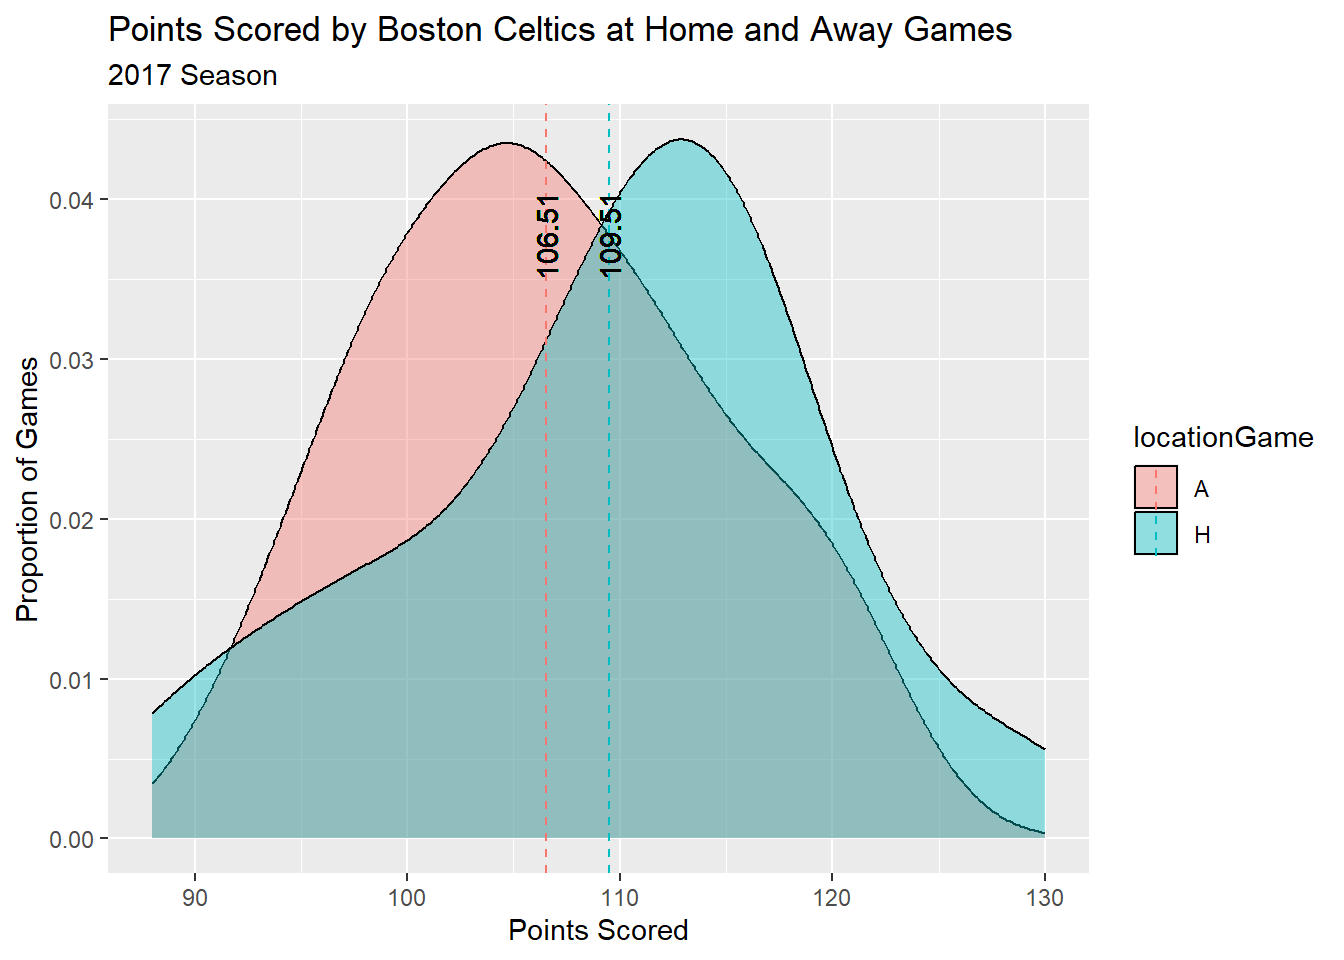
\includegraphics{4_Uni_Multivariate_PS4_files/figure-latex/unnamed-chunk-3-1.pdf}

\begin{quote}
We see the Boston Celtics have an average of 106.5122 pts scored at away
games (A), and and average of 109.5122 pts scored at home games (H).
Since we're visualizing a continuous variable, we want to use a densty
curve.
\end{quote}

\hypertarget{question-2-1-point}{%
\subsection{Question 2 {[}1 point{]}}\label{question-2-1-point}}

Now recreate the same plot for the 2018, 2019, and combined seasons.
Imagine that you work for the Celtics organization and Brad Stevens (the
GM), asks you if the team scores more points at home or away? Based on
your analysis, what would you tell him?

\begin{Shaded}
\begin{Highlighting}[]
\CommentTok{\# By season}
\NormalTok{games }\SpecialCharTok{\%\textgreater{}\%}
  \FunctionTok{filter}\NormalTok{(nameTeam}\SpecialCharTok{==}\StringTok{"Boston Celtics"}\NormalTok{) }\SpecialCharTok{\%\textgreater{}\%} \CommentTok{\# Filter to the Boston Celtics (nameTeam)}
  \FunctionTok{group\_by}\NormalTok{(locationGame, yearSeason) }\SpecialCharTok{\%\textgreater{}\%} \CommentTok{\# Group by the location (locationGame) and the season (yearSeason)}
  \FunctionTok{summarise}\NormalTok{(}\AttributeTok{avg\_pts=}\FunctionTok{mean}\NormalTok{(pts)) }\CommentTok{\# Calculate the average points (pts)}
\end{Highlighting}
\end{Shaded}

\begin{verbatim}
## `summarise()` has grouped output by 'locationGame'. You can override using the
## `.groups` argument.
\end{verbatim}

\begin{verbatim}
## # A tibble: 6 x 3
## # Groups:   locationGame [2]
##   locationGame yearSeason avg_pts
##   <chr>             <int>   <dbl>
## 1 A                  2017    107.
## 2 A                  2018    103.
## 3 A                  2019    111.
## 4 H                  2017    110.
## 5 H                  2018    105.
## 6 H                  2019    114.
\end{verbatim}

\begin{Shaded}
\begin{Highlighting}[]
\NormalTok{games\_data2 }\OtherTok{\textless{}{-}}\NormalTok{ games }\SpecialCharTok{\%\textgreater{}\%}
  \FunctionTok{filter}\NormalTok{(nameTeam}\SpecialCharTok{==}\StringTok{"Boston Celtics"}\NormalTok{) }\SpecialCharTok{\%\textgreater{}\%}
  \FunctionTok{group\_by}\NormalTok{(locationGame, yearSeason) }\SpecialCharTok{\%\textgreater{}\%}
  \FunctionTok{mutate}\NormalTok{(}\AttributeTok{avg\_pts=}\FunctionTok{mean}\NormalTok{(pts))}
  
\NormalTok{games }\SpecialCharTok{\%\textgreater{}\%}
  \FunctionTok{filter}\NormalTok{(nameTeam}\SpecialCharTok{==}\StringTok{"Boston Celtics"}\NormalTok{) }\SpecialCharTok{\%\textgreater{}\%} \CommentTok{\# Filter to the Boston Celtics (nameTeam)}
  \FunctionTok{ggplot}\NormalTok{(}\FunctionTok{aes}\NormalTok{(}\AttributeTok{x=}\NormalTok{pts, }\AttributeTok{fill=}\NormalTok{locationGame)) }\SpecialCharTok{+} \CommentTok{\# Create a multivariate plot comparing points scored between home and away games}
  \FunctionTok{geom\_density}\NormalTok{(}\AttributeTok{alpha=}\FloatTok{0.4}\NormalTok{) }\SpecialCharTok{+} \CommentTok{\# Choose the appropriate geom\_... for this plot (i.e., geom\_histogram(), geom\_density(), geom\_bar(), etc.)}
  \FunctionTok{labs}\NormalTok{(}\AttributeTok{title=}\StringTok{"Points Scored by Boston Celtics at Home and Away Games"}\NormalTok{,}
       \AttributeTok{subtitle=}\StringTok{"2017{-}2019 Season"}\NormalTok{,}
       \AttributeTok{x=}\StringTok{"Points Scored"}\NormalTok{,}
       \AttributeTok{y=}\StringTok{"Proportion of Games"}\NormalTok{) }\SpecialCharTok{+} \CommentTok{\# Add clear descriptions for the title, subtitle, axes, and legend}
  \FunctionTok{facet\_wrap}\NormalTok{(}\SpecialCharTok{\textasciitilde{}}\NormalTok{ yearSeason) }\SpecialCharTok{+} \CommentTok{\# Create separate panels for each season (facet\_wrap())}
  \FunctionTok{geom\_vline}\NormalTok{(}\AttributeTok{data=}\NormalTok{games\_data2, }\FunctionTok{aes}\NormalTok{(}\AttributeTok{xintercept=}\NormalTok{avg\_pts, }\AttributeTok{color=}\NormalTok{locationGame), }\AttributeTok{linetype=}\StringTok{"dashed"}\NormalTok{) }
\end{Highlighting}
\end{Shaded}

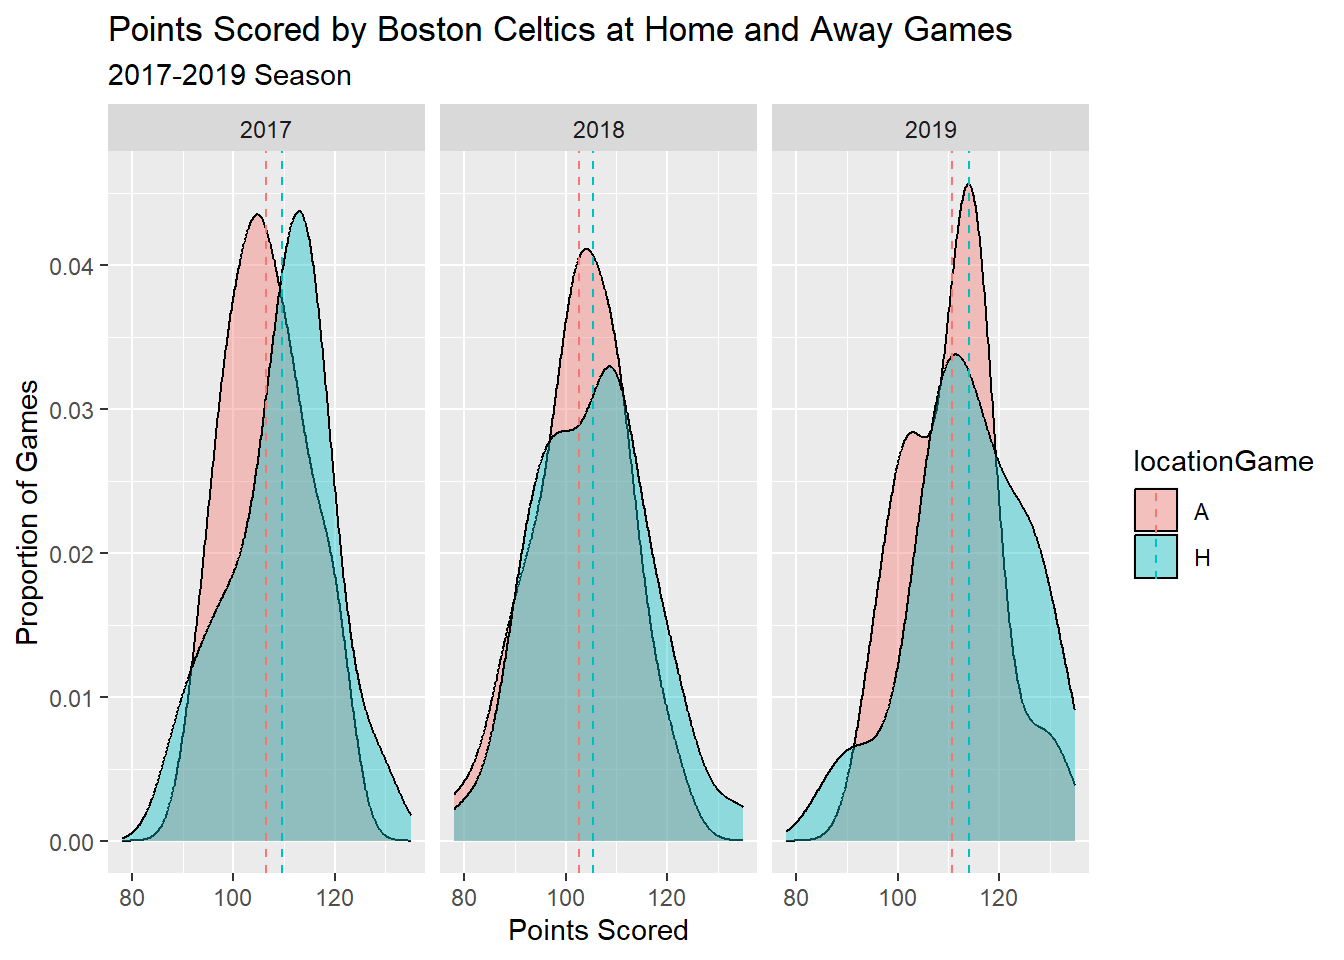
\includegraphics{4_Uni_Multivariate_PS4_files/figure-latex/unnamed-chunk-4-1.pdf}

\begin{Shaded}
\begin{Highlighting}[]
\CommentTok{\# Over all seasons combined}
\NormalTok{games }\SpecialCharTok{\%\textgreater{}\%}
  \FunctionTok{filter}\NormalTok{(nameTeam}\SpecialCharTok{==}\StringTok{"Boston Celtics"}\NormalTok{) }\SpecialCharTok{\%\textgreater{}\%} \CommentTok{\# Filter to the Boston Celtics (nameTeam)}
  \FunctionTok{group\_by}\NormalTok{(locationGame) }\SpecialCharTok{\%\textgreater{}\%} \CommentTok{\# Group by the location (locationGame)}
  \FunctionTok{summarise}\NormalTok{(}\AttributeTok{avg\_pts=}\FunctionTok{mean}\NormalTok{(pts)) }\CommentTok{\# Calculate the average points (pts)}
\end{Highlighting}
\end{Shaded}

\begin{verbatim}
## # A tibble: 2 x 2
##   locationGame avg_pts
##   <chr>          <dbl>
## 1 A               107.
## 2 H               110.
\end{verbatim}

\begin{Shaded}
\begin{Highlighting}[]
\NormalTok{games\_ov }\OtherTok{\textless{}{-}}\NormalTok{ games }\SpecialCharTok{\%\textgreater{}\%}
  \FunctionTok{filter}\NormalTok{(nameTeam}\SpecialCharTok{==}\StringTok{"Boston Celtics"}\NormalTok{) }\SpecialCharTok{\%\textgreater{}\%}
  \FunctionTok{group\_by}\NormalTok{(locationGame) }\SpecialCharTok{\%\textgreater{}\%}
  \FunctionTok{mutate}\NormalTok{(}\AttributeTok{avg\_pts=}\FunctionTok{mean}\NormalTok{(pts))}

\NormalTok{games }\SpecialCharTok{\%\textgreater{}\%}
  \FunctionTok{filter}\NormalTok{(nameTeam}\SpecialCharTok{==}\StringTok{"Boston Celtics"}\NormalTok{) }\SpecialCharTok{\%\textgreater{}\%} \CommentTok{\# Filter to the Boston Celtics (nameTeam)}
  \FunctionTok{ggplot}\NormalTok{(}\FunctionTok{aes}\NormalTok{(}\AttributeTok{x=}\NormalTok{pts, }\AttributeTok{fill=}\NormalTok{locationGame)) }\SpecialCharTok{+} \CommentTok{\# Create a multivariate plot comparing points scored between home and away games}
  \FunctionTok{geom\_density}\NormalTok{(}\AttributeTok{alpha=}\FloatTok{0.4}\NormalTok{) }\SpecialCharTok{+} \CommentTok{\# Choose the appropriate geom\_... for this plot (i.e., geom\_histogram(), geom\_density(), geom\_bar(), etc.)}
  \FunctionTok{labs}\NormalTok{(}\AttributeTok{title=}\StringTok{"Points Scored by Boston Celtics at Home and Away Games"}\NormalTok{,}
       \AttributeTok{subtitle=}\StringTok{"All Seasons"}\NormalTok{,}
       \AttributeTok{x=}\StringTok{"Points Scored"}\NormalTok{,}
       \AttributeTok{y=}\StringTok{"Proportion of Games"}\NormalTok{) }\SpecialCharTok{+} \CommentTok{\# Add clear descriptions for the title, subtitle, axes, and legend}
  \FunctionTok{geom\_vline}\NormalTok{(}\AttributeTok{data=}\NormalTok{games\_ov, }\FunctionTok{aes}\NormalTok{(}\AttributeTok{xintercept=}\NormalTok{avg\_pts, }\AttributeTok{color=}\NormalTok{locationGame), }\AttributeTok{linetype=}\StringTok{"dashed"}\NormalTok{) }
\end{Highlighting}
\end{Shaded}

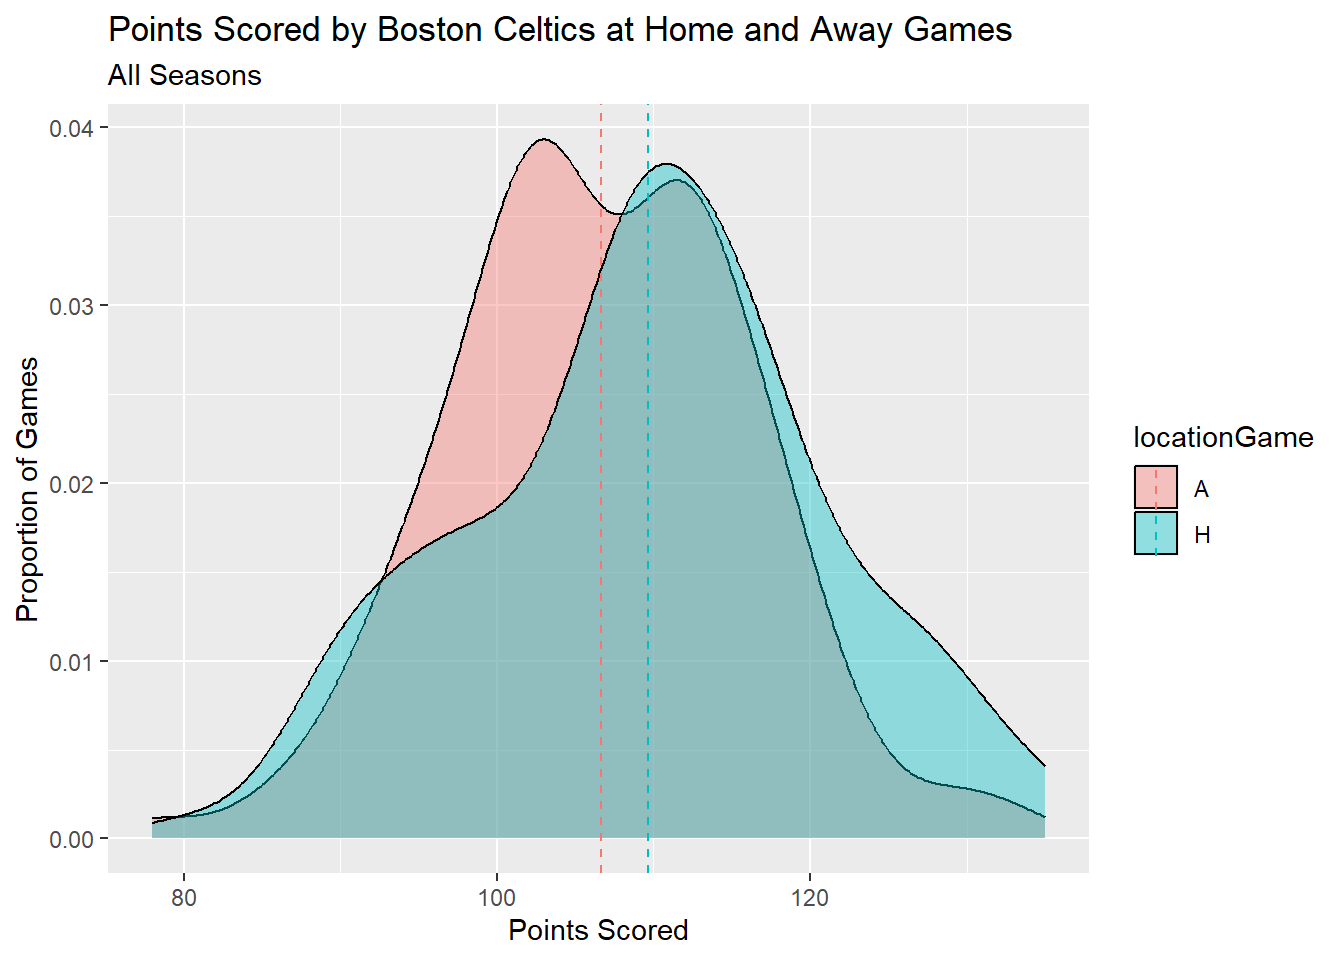
\includegraphics{4_Uni_Multivariate_PS4_files/figure-latex/unnamed-chunk-4-2.pdf}

\begin{quote}
The average home game sees a more points scored than away games.
However, fewer games were played at home during the 2018 and 2019
seasons-- allowing outliers to have a greater influence on the average
points variable. Looking at all seasons, though, our conclusion that
more points are scored at home than away.
\end{quote}

\hypertarget{question-3-2-points-1-ec}{%
\subsection{Question 3 {[}2 points + 1
EC{]}}\label{question-3-2-points-1-ec}}

Brad Stevens thanks you for your answer, but is a well-trained
statistician in his own right, and wants to know how confident you are
in your claim. Bootstrap sample the data 1,000 times to provide him with
a more sophisticated answer. How confident are you in your conclusion
that the Celtics score more points at home games than away games? Make
sure to \texttt{set.seed(123)} to ensure you get the same answer every
time you \texttt{knit} your code! EC: Visualize your answer.

\begin{Shaded}
\begin{Highlighting}[]
\CommentTok{\# Set the seed!}
\FunctionTok{set.seed}\NormalTok{(}\DecValTok{123}\NormalTok{)}
\NormalTok{forBS }\OtherTok{\textless{}{-}}\NormalTok{ games }\SpecialCharTok{\%\textgreater{}\%} \CommentTok{\# To make things easier, create a new data object that is filtered to just the Celtics}
    \FunctionTok{filter}\NormalTok{(nameTeam}\SpecialCharTok{==}\StringTok{"Boston Celtics"}\NormalTok{) }\CommentTok{\# Filter to the Celtics (nameTeam)}

\NormalTok{bsRes }\OtherTok{\textless{}{-}} \ConstantTok{NULL} \CommentTok{\# Instantiate an empty object to store data from the loop}
\ControlFlowTok{for}\NormalTok{(i }\ControlFlowTok{in} \DecValTok{1}\SpecialCharTok{:}\DecValTok{1000}\NormalTok{) \{ }\CommentTok{\# Loop 1,000 times}
\NormalTok{  bsRes }\OtherTok{\textless{}{-}}\NormalTok{ forBS }\SpecialCharTok{\%\textgreater{}\%}
    \FunctionTok{sample\_n}\NormalTok{(}\AttributeTok{size=}\FunctionTok{nrow}\NormalTok{(forBS),}\AttributeTok{replace=}\NormalTok{T) }\SpecialCharTok{\%\textgreater{}\%} \CommentTok{\# Sample the data with replacement using all possible rows}
    \FunctionTok{group\_by}\NormalTok{(locationGame) }\SpecialCharTok{\%\textgreater{}\%} \CommentTok{\# Group by the location of the game (locationGame)}
    \FunctionTok{summarise}\NormalTok{(}\AttributeTok{avg\_pts=}\FunctionTok{mean}\NormalTok{(pts)) }\SpecialCharTok{\%\textgreater{}\%} \CommentTok{\# Calculate the average points (pts)}
    \FunctionTok{ungroup}\NormalTok{() }\SpecialCharTok{\%\textgreater{}\%} \CommentTok{\# Best practices!}
    \FunctionTok{spread}\NormalTok{(}\AttributeTok{key=}\NormalTok{locationGame, }\AttributeTok{value=}\NormalTok{avg\_pts) }\SpecialCharTok{\%\textgreater{}\%} \CommentTok{\# Spread the data to get one column for average points at home and another for average points away}
    \FunctionTok{mutate}\NormalTok{(}\AttributeTok{diff =}\NormalTok{ H}\SpecialCharTok{{-}}\NormalTok{A, }\CommentTok{\# Calculate the difference between home and away points}
           \AttributeTok{bsInd =}\NormalTok{ i) }\SpecialCharTok{\%\textgreater{}\%} \CommentTok{\# Save the bootstrap index}
    \FunctionTok{bind\_rows}\NormalTok{(bsRes) }\CommentTok{\# Append the result to the empty object from line 133}
\NormalTok{\} }

\CommentTok{\# Calculate the confidence}
\NormalTok{bsRes }\SpecialCharTok{\%\textgreater{}\%}
  \FunctionTok{summarise}\NormalTok{(}\AttributeTok{confidence =} \FunctionTok{mean}\NormalTok{(diff}\SpecialCharTok{\textgreater{}}\DecValTok{0}\NormalTok{, }\AttributeTok{na.rm=}\NormalTok{T), }\CommentTok{\# Calculate the proportion of bootstrap simulations where the home points are greater than the away points}
            \AttributeTok{avg\_diff =} \FunctionTok{mean}\NormalTok{(diff, }\AttributeTok{na.rm=}\NormalTok{T)) }\CommentTok{\# Calculate the overall average difference}
\end{Highlighting}
\end{Shaded}

\begin{verbatim}
## # A tibble: 1 x 2
##   confidence avg_diff
##        <dbl>    <dbl>
## 1      0.992     2.93
\end{verbatim}

\begin{Shaded}
\begin{Highlighting}[]
\CommentTok{\# EC: Plot the result}
\end{Highlighting}
\end{Shaded}

\begin{quote}
Supporting our earlier claim, we are 99.2\% confident that the Celtics
have a homecourt advantage.
\end{quote}

\hypertarget{question-4-2-point-1-ec}{%
\subsection{Question 4 {[}2 point + 1
EC{]}}\label{question-4-2-point-1-ec}}

Re-do this analysis for three other statistics of interest to Brad:
total rebounds (\texttt{treb}), turnovers (\texttt{tov}), and field goal
percent (\texttt{pctFG}). EC: theorize about the seeming paradox in your
answer to Brad Stevens.

\begin{Shaded}
\begin{Highlighting}[]
\FunctionTok{set.seed}\NormalTok{(}\DecValTok{123}\NormalTok{)}
\NormalTok{forBS }\OtherTok{\textless{}{-}}\NormalTok{ games }\SpecialCharTok{\%\textgreater{}\%} \CommentTok{\# To make things easier, create a new data object that is filtered to just the Celtics}
    \FunctionTok{filter}\NormalTok{(nameTeam}\SpecialCharTok{==}\StringTok{"Boston Celtics"}\NormalTok{) }\CommentTok{\# Filter to the Celtics (nameTeam)}

\NormalTok{bsRes }\OtherTok{\textless{}{-}} \ConstantTok{NULL} \CommentTok{\# Instantiate an empty object to store data from the loop}
\ControlFlowTok{for}\NormalTok{(i }\ControlFlowTok{in} \DecValTok{1}\SpecialCharTok{:}\DecValTok{1000}\NormalTok{) \{ }\CommentTok{\# Loop 1,000 times}
\NormalTok{  bsRes }\OtherTok{\textless{}{-}}\NormalTok{ forBS }\SpecialCharTok{\%\textgreater{}\%}
    \FunctionTok{sample\_n}\NormalTok{(}\AttributeTok{size=}\FunctionTok{n}\NormalTok{(), }\AttributeTok{replace =}\NormalTok{ T) }\SpecialCharTok{\%\textgreater{}\%} \CommentTok{\# Sample the data with replacement using all possible rows}
    \FunctionTok{group\_by}\NormalTok{(locationGame) }\SpecialCharTok{\%\textgreater{}\%} \CommentTok{\# Group by the location of the game (locationGame)}
    \FunctionTok{summarise}\NormalTok{(}\AttributeTok{avg\_reb =} \FunctionTok{mean}\NormalTok{(treb), }\CommentTok{\# Calculate the average total rebounds (treb)}
              \AttributeTok{avg\_tov =} \FunctionTok{mean}\NormalTok{(tov), }\CommentTok{\# Calculate the average turnovers (tov)}
              \AttributeTok{avg\_pctFG =} \FunctionTok{mean}\NormalTok{(pctFG)) }\SpecialCharTok{\%\textgreater{}\%} \CommentTok{\# Calculate the average field goal shooting percentage (pctFG)}
    \FunctionTok{ungroup}\NormalTok{() }\SpecialCharTok{\%\textgreater{}\%} \CommentTok{\# Best practices!}
    \FunctionTok{pivot\_wider}\NormalTok{(}\AttributeTok{names\_from =}\NormalTok{ locationGame, }\CommentTok{\# Pivot wider to get each measure in its own column for home and away games.}
                \AttributeTok{values\_from =} \FunctionTok{c}\NormalTok{(avg\_reb, avg\_tov, avg\_pctFG)) }\SpecialCharTok{\%\textgreater{}\%} \CommentTok{\# Use the values from the variables you created above}
    \FunctionTok{mutate}\NormalTok{(}\AttributeTok{diff\_reb =}\NormalTok{ avg\_reb\_H}\SpecialCharTok{{-}}\NormalTok{avg\_reb\_A, }\CommentTok{\# Calculate the difference between home and away total rebounds}
           \AttributeTok{diff\_tov =}\NormalTok{ avg\_tov\_H}\SpecialCharTok{{-}}\NormalTok{avg\_tov\_A, }\CommentTok{\# Calculate the difference between home and away turnovers}
           \AttributeTok{diff\_pctFG =}\NormalTok{ avg\_pctFG\_H}\SpecialCharTok{{-}}\NormalTok{avg\_pctFG\_A, }\CommentTok{\# Calculate the difference between home and away field goal percentages}
           \AttributeTok{bsInd =}\NormalTok{ i) }\SpecialCharTok{\%\textgreater{}\%} \CommentTok{\# Save the bootstrap index}
    \FunctionTok{bind\_rows}\NormalTok{(bsRes) }\CommentTok{\# Append the result to the empty object from line 165}
\NormalTok{\} }

\CommentTok{\# Calculate the confidence}
\NormalTok{bsRes }\SpecialCharTok{\%\textgreater{}\%}
  \FunctionTok{summarise}\NormalTok{(}\AttributeTok{confidence\_reb =} \FunctionTok{mean}\NormalTok{(diff\_reb}\SpecialCharTok{\textgreater{}}\DecValTok{0}\NormalTok{, }\AttributeTok{na.rm=}\NormalTok{T), }\CommentTok{\# Calculate the confidence for the home court advantage in rebounds}
            \AttributeTok{confidence\_tov =} \FunctionTok{mean}\NormalTok{(diff\_tov}\SpecialCharTok{\textgreater{}}\DecValTok{0}\NormalTok{, }\AttributeTok{na.rm=}\NormalTok{T), }\CommentTok{\# Calculate the confidence for the home court (dis)advantage in turnovers}
            \AttributeTok{confidence\_pctFG =} \FunctionTok{mean}\NormalTok{(diff\_pctFG}\SpecialCharTok{\textgreater{}}\DecValTok{0}\NormalTok{, }\AttributeTok{na.rm=}\NormalTok{T)) }\CommentTok{\# Calculate the confidence for the home court advantage in FG\%}
\end{Highlighting}
\end{Shaded}

\begin{verbatim}
## # A tibble: 1 x 3
##   confidence_reb confidence_tov confidence_pctFG
##            <dbl>          <dbl>            <dbl>
## 1          0.999          0.942              0.9
\end{verbatim}

\begin{quote}
We are 99.9\% confident in our home court advantage in rebounds, and
90\% confident in our home court advantage in field goal percentage, but
we surprisingly have 94.2\% confidence attached to our turnover
variable. This would imply a home court disadvtange, as the Celtics
frequently lose the ball at home. How could we have a home court
advantage if we never have the ball?
\end{quote}

\hypertarget{question-5-2-point-1-ec}{%
\subsection{Question 5 {[}2 point + 1
EC{]}}\label{question-5-2-point-1-ec}}

Now Brad is asking for a similar analysis of other teams. Calculate the
difference between home and away turnovers for every team in the league
and prepare a summary table that includes both the average difference
for each team, as well as your confidence about the difference is not
zero. Based on these data, would you argue that there is an
\textbf{overall} home court advantage in terms of turnovers across the
NBA writ large? EC \#1: visualize these summary results by plotting the
difference on the x-axis, the teams (reordered) on the y-axis, and the
points colored by whether you are more than 90\% confident in your
answer. EC \#2: How should we interpret confidence levels less than
50\%?

\begin{Shaded}
\begin{Highlighting}[]
\FunctionTok{set.seed}\NormalTok{(}\DecValTok{123}\NormalTok{)}
\NormalTok{bsRes }\OtherTok{\textless{}{-}} \ConstantTok{NULL} \CommentTok{\# Instantiate an empty object to store data from the loop}
\ControlFlowTok{for}\NormalTok{(i }\ControlFlowTok{in} \DecValTok{1}\SpecialCharTok{:}\DecValTok{1000}\NormalTok{) \{ }\CommentTok{\# Loop 1,000 times}
\NormalTok{  bsRes }\OtherTok{\textless{}{-}}\NormalTok{ games }\SpecialCharTok{\%\textgreater{}\%}
    \FunctionTok{group\_by}\NormalTok{(nameTeam) }\SpecialCharTok{\%\textgreater{}\%} \CommentTok{\# Group by the team (nameTeam)}
    \FunctionTok{sample\_n}\NormalTok{(}\AttributeTok{size=}\FunctionTok{n}\NormalTok{(), }\AttributeTok{replace=}\NormalTok{T) }\SpecialCharTok{\%\textgreater{}\%} \CommentTok{\# Sample the data with replacement using all possible rows FOR EACH TEAM (hint: use n())}
    \FunctionTok{group\_by}\NormalTok{(locationGame, nameTeam) }\SpecialCharTok{\%\textgreater{}\%} \CommentTok{\# Group by the location of the game (locationGame) and the team (nameTeam)}
    \FunctionTok{summarise}\NormalTok{(}\AttributeTok{avg\_tov =} \FunctionTok{mean}\NormalTok{(tov, }\AttributeTok{na.rm=}\NormalTok{T), }\CommentTok{\# Calculate the average turnovers (tov)}
              \AttributeTok{.groups =} \StringTok{\textquotesingle{}drop\textquotesingle{}}\NormalTok{) }\SpecialCharTok{\%\textgreater{}\%} \CommentTok{\# Best practices! (Also reduces the messages!)}
    \FunctionTok{pivot\_wider}\NormalTok{(}\AttributeTok{id\_cols =}\NormalTok{ nameTeam, }\CommentTok{\# Set the ID colunm to the team (nameTeam)}
                \AttributeTok{names\_from =}\NormalTok{ locationGame, }\CommentTok{\# Pivot wider to get each measure in its own column for home and away games}
                \AttributeTok{values\_from =} \FunctionTok{c}\NormalTok{(}\StringTok{\textquotesingle{}avg\_tov\textquotesingle{}}\NormalTok{)) }\SpecialCharTok{\%\textgreater{}\%} \CommentTok{\# Use the values from the average turnover measure you created above}
    \FunctionTok{mutate}\NormalTok{(}\AttributeTok{diff\_tov =}\NormalTok{ H}\SpecialCharTok{{-}}\NormalTok{A, }\CommentTok{\# Calculate the difference between home and away turnovers}
           \AttributeTok{bsInd =}\NormalTok{ i) }\SpecialCharTok{\%\textgreater{}\%} \CommentTok{\# Save the bootstrap index}
    \FunctionTok{bind\_rows}\NormalTok{(bsRes) }\CommentTok{\# Append the result to the empty object from line 165}
\NormalTok{\} }

\NormalTok{bsRes }\SpecialCharTok{\%\textgreater{}\%} \CommentTok{\# If you want to attempt the EC\#1, it helps to save the summarized results to a new object \textquotesingle{}toplot\textquotesingle{}}
  \FunctionTok{group\_by}\NormalTok{(nameTeam) }\SpecialCharTok{\%\textgreater{}\%} \CommentTok{\# Group by the team (nameTeam)}
  \FunctionTok{summarise}\NormalTok{(}\AttributeTok{conf\_tov =} \FunctionTok{round}\NormalTok{(}\FunctionTok{mean}\NormalTok{(diff\_tov}\SpecialCharTok{\textgreater{}}\DecValTok{0}\NormalTok{), }\DecValTok{2}\NormalTok{), }\CommentTok{\# Calculate the confidence and round the number to two digits}
            \AttributeTok{diff\_tov =} \FunctionTok{round}\NormalTok{(}\FunctionTok{mean}\NormalTok{(diff\_tov), }\DecValTok{2}\NormalTok{)) }\CommentTok{\# Calculate the average difference and round the number to two digits}
\end{Highlighting}
\end{Shaded}

\begin{verbatim}
## # A tibble: 30 x 3
##    nameTeam              conf_tov diff_tov
##    <chr>                    <dbl>    <dbl>
##  1 Atlanta Hawks             0.02    -0.98
##  2 Boston Celtics            0.94     0.63
##  3 Brooklyn Nets             0.38    -0.14
##  4 Charlotte Hornets         0.56     0.07
##  5 Chicago Bulls             0.02    -0.99
##  6 Cleveland Cavaliers       0.43    -0.09
##  7 Dallas Mavericks          0.68     0.23
##  8 Denver Nuggets            0.25    -0.34
##  9 Detroit Pistons           0.56     0.07
## 10 Golden State Warriors     0.8      0.39
## # ... with 20 more rows
\end{verbatim}

\begin{Shaded}
\begin{Highlighting}[]
\CommentTok{\# EC \#1: Visualize the results. Make sure to label clearly!}
\end{Highlighting}
\end{Shaded}

\begin{quote}
Analyzing the data, we find the average difference between home
turnovers and away turnovers is negative, indicating that for most
teams, turnovers occur more often at away games. That said, the
confidence associated with each negative `diff\_tov' value is low,
establishing that we are not confident about this relationship between
turnovers at away games. Looking at the positive `diff\_tov' values
(which indicates more turnovers happened at home games), we have a much
higher confidence, establishing that we are confident in our conclusion
regarding greater turnovers at home games. Therefore, we can't conclude
a home court advantage exists.
\end{quote}

\hypertarget{question-6-2-points}{%
\subsection{Question 6 {[}2 points{]}}\label{question-6-2-points}}

Redo question 5 but analyze the point difference instead. Do you think
there is a systematic home court advantage in terms of points across the
NBA writ large?

\begin{Shaded}
\begin{Highlighting}[]
\FunctionTok{set.seed}\NormalTok{(}\DecValTok{123}\NormalTok{)}
\NormalTok{bsRes }\OtherTok{\textless{}{-}} \ConstantTok{NULL} \CommentTok{\# Instantiate an empty object to store data from the loop}
\ControlFlowTok{for}\NormalTok{(i }\ControlFlowTok{in} \DecValTok{1}\SpecialCharTok{:}\DecValTok{1000}\NormalTok{) \{ }\CommentTok{\# Loop 1,000 times}
\NormalTok{  bsRes }\OtherTok{\textless{}{-}}\NormalTok{ games }\SpecialCharTok{\%\textgreater{}\%}
    \FunctionTok{group\_by}\NormalTok{(nameTeam) }\SpecialCharTok{\%\textgreater{}\%} \CommentTok{\# Group by the team (nameTeam)}
    \FunctionTok{sample\_n}\NormalTok{(}\AttributeTok{size=}\FunctionTok{n}\NormalTok{(), }\AttributeTok{replace=}\NormalTok{T) }\SpecialCharTok{\%\textgreater{}\%} \CommentTok{\# Sample the data with replacement using all possible rows FOR EACH TEAM (hint: use n())}
    \FunctionTok{group\_by}\NormalTok{(locationGame, nameTeam) }\SpecialCharTok{\%\textgreater{}\%} \CommentTok{\# Group by the location of the game (locationGame) and the team (nameTeam)}
    \FunctionTok{summarise}\NormalTok{(}\AttributeTok{avg\_pts =} \FunctionTok{mean}\NormalTok{(pts, }\AttributeTok{na.rm=}\NormalTok{T), }\CommentTok{\# Calculate the average turnovers (tov)}
              \AttributeTok{.groups =} \StringTok{\textquotesingle{}drop\textquotesingle{}}\NormalTok{) }\SpecialCharTok{\%\textgreater{}\%} \CommentTok{\# Best practices! (Also reduces the messages!)}
    \FunctionTok{pivot\_wider}\NormalTok{(}\AttributeTok{id\_cols =}\NormalTok{ nameTeam, }\CommentTok{\# Set the ID colunm to the team (nameTeam)}
                \AttributeTok{names\_from =}\NormalTok{ locationGame, }\CommentTok{\# Pivot wider to get each measure in its own column for home and away games}
                \AttributeTok{values\_from =} \FunctionTok{c}\NormalTok{(}\StringTok{\textquotesingle{}avg\_pts\textquotesingle{}}\NormalTok{)) }\SpecialCharTok{\%\textgreater{}\%} \CommentTok{\# Use the values from the average turnover measure you created above}
    \FunctionTok{mutate}\NormalTok{(}\AttributeTok{diff\_pts =}\NormalTok{ H}\SpecialCharTok{{-}}\NormalTok{A, }\CommentTok{\# Calculate the difference between home and away turnovers}
           \AttributeTok{bsInd =}\NormalTok{ i) }\SpecialCharTok{\%\textgreater{}\%} \CommentTok{\# Save the bootstrap index}
    \FunctionTok{bind\_rows}\NormalTok{(bsRes) }\CommentTok{\# Append the result to the empty object from line 165}
\NormalTok{\} }

\NormalTok{bsRes }\SpecialCharTok{\%\textgreater{}\%} \CommentTok{\# If you want to attempt the EC\#1, it helps to save the summarized results to a new object \textquotesingle{}toplot\textquotesingle{}}
  \FunctionTok{group\_by}\NormalTok{(nameTeam) }\SpecialCharTok{\%\textgreater{}\%} \CommentTok{\# Group by the team (nameTeam)}
  \FunctionTok{summarise}\NormalTok{(}\AttributeTok{conf\_pts =} \FunctionTok{round}\NormalTok{(}\FunctionTok{mean}\NormalTok{(diff\_pts}\SpecialCharTok{\textgreater{}}\DecValTok{0}\NormalTok{), }\DecValTok{2}\NormalTok{), }\CommentTok{\# Calculate the confidence and round the number to two digits}
            \AttributeTok{diff\_pts =} \FunctionTok{round}\NormalTok{(}\FunctionTok{mean}\NormalTok{(diff\_pts), }\DecValTok{2}\NormalTok{)) }\CommentTok{\# Calculate the average difference and round the number to two digits}
\end{Highlighting}
\end{Shaded}

\begin{verbatim}
## # A tibble: 30 x 3
##    nameTeam              conf_pts diff_pts
##    <chr>                    <dbl>    <dbl>
##  1 Atlanta Hawks             1        4.37
##  2 Boston Celtics            0.99     3.01
##  3 Brooklyn Nets             0.42    -0.43
##  4 Charlotte Hornets         0.99     3.86
##  5 Chicago Bulls             0.49    -0.04
##  6 Cleveland Cavaliers       0.94     2.45
##  7 Dallas Mavericks          0.98     2.99
##  8 Denver Nuggets            1        4.88
##  9 Detroit Pistons           0.99     3.41
## 10 Golden State Warriors     0.9      2.04
## # ... with 20 more rows
\end{verbatim}

\begin{quote}
The difference in points indicates a home court advantage, which is
accompanied by high confidence for each `diff\_pts' variable.
\end{quote}

\end{document}
